\documentclass[UTF8]{ctexart}

\usepackage{subfiles}  

%下面的语句, 引入你的头部设置文件
\usepackage{C:/phpStorm_proj/02_myself_ID_EGO/+100_latex_all_math_sel/myPreamble} 
%必须是绝对路径,才能让各个tex在单独编译时使用到

\title{文件名}


%---------------------------------


\begin{document}
	\tableofcontents % 生成目录
	\date{} % 若不写这句, 则默认也会渲染出日期, 所以我们要手动赋空值
	\maketitle  %这行代码, 让你前面的 title, author, date生效
	
	
	
	
	\section{离散型数据 - 概率函数 (概率质量函数) : Probability mass function (PMF)}
	
	描述``离散型数据"的概率分布情况 的曲线, 称为``概率质量函数"(PMF). \\
	
	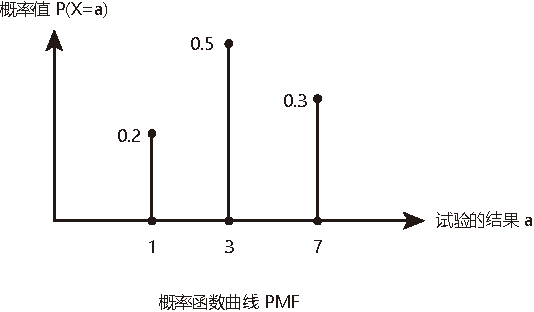
\includegraphics[width=0.6\textwidth]{/0116.pdf} \\
	
	比如,掷骰子, 不同点朝上的概率为:$
	\underset{\text{骰子在第}i\text{点的概率}}{\underbrace{p_i}}=\underset{\text{随机变量}X\text{在第}i\text{点时的概率}}{\underbrace{P(X=a_i)}},\ \ i\in 1,2,3,4,5,6
	$ \\
	
	在上面这个函数里 : \\
	- 自变量X : 是``随机变量"的取值. \\
	- 因变量  $ p_i$ 是``自变量X所取到某个值 $a_i$"的概率. \\
	
	从公式上来看, \textbf{``概率函数", 一次只能表示一个取值的概率.} 比如 $ P(X=1)= 1/6$ 就表示: 当随机变量X 取值为 1时 (即骰子投到点数为1时) 的概率为1/6. 所以说, 它一次只能代表``随机变量的一个取值"的概率. \textbf{(即: P后面的小括号里, 只能写成 X= ..., 而不能写成 X>... 或 X<..., 大于小于符号这些, 就是属于``累加函数"了.)}\\
	
	
	
	典型的``离散概率分布"包括: 伯努利分布,二项分布,几何分布,泊松分布等. 
	
	
	~\\
	\hrule
	~\\
	
	
	\section{连续型数据 - 概率函数 (概率密度函数) : Probability Density function (PDF)}
	
	``连续型数据"的概率分布, 称为``概率密度函数"(PDF).  \\
	
	
	``概率密度函数"的 某区间上的概率值 = 该区间的函数曲线段, 与x坐标轴之间围成的面积. 实际上就是对``概率密度函数"进行定积分. \\
	
	
	$\int_{ - \infty }^{ + \infty } \text{概率函数}f(x)dx = 1$ \\
	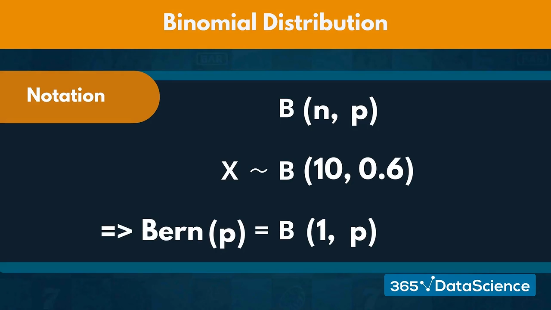
\includegraphics[width=0.5\textwidth]{/0126.png} \\
	
	
	\begin{myEnvSample}
		有概率函数 $
		f\left( x \right) =\left\{ \begin{array}{l}
			kx+1\ \ \left( 0\leq x\leq 2 \right)\\
			0\ \ \ \ \ \ \ \ \left( x\text{是其他的话} \right)\\
		\end{array} \right. 
		$ \\
		
		(1)求k. \\
		根据``概率密度函数 f(x)"的性质, 有 $\int_{-\infty}^{+\infty}{f\left( x \right)} dx=1$. \\
		既然本题中, x只在(0,2)区间上才有概率值(=kx+1); 而在其他定义域区间上, 概率值都是=0. 这就说明, 该概率函数的全部概率值(``求和=1"), 就只在(0,2)区间上. \\
		
		即:
		\begin{align*}  % 支持每行编号. 若不需要编号, 就用 align*环境
			&\int_0^2{\left( kx+1 \right)}dx=1\\
			&\int_0^2{\left( \underset{\text{可视为常数}}{\underbrace{k}}x \right)}dx+\int_0^2{1}dx=1\\
			&k\left( \frac{1}{1+1}x^{1+1}\mid_{0}^{2} \right) +x\mid_{0}^{2}=1\\
			&k\left( \frac{x^2}{2}\mid_{0}^{2} \right) +2=1\\
			&k\frac{2^2}{2}+2=1\\
			&k=-\frac{1}{2}
		\end{align*} 
		
		
		
		(2)求
		\begin{align*}  % 支持每行编号. 若不需要编号, 就用 align*环境
			&P\left\{ x\leq 2 \right\}  \\
			&=P\left\{ -\infty <x<2 \right\}\\
			&	=\int_{-\infty}^2{\underset{=kx+1,\text{而}k\text{上面已算出}=-\frac{1}{2}}{\underbrace{f\left( x \right) }}}dx\\\
			&	\text{← 因为}x\text{只在}\left( 0,2 \right) \text{区间上有值,所以本处的}\left( -\infty ,2 \right) \text{其实就可直接写成}\left( 0,2 \right)\\
			&	=\int_{-\infty}^2{\left( -\frac{1}{2}x+1 \right)}dx=1
		\end{align*}
		
		
		
		(3)求 
		\begin{align*}  % 支持每行编号. 若不需要编号, 就用 align*环境
			&	P\left\{ 1.5<x<2.5 \right\} \\
			&=\int_{1.5}^{2.5}{\underset{=kx+1,\text{而}k\text{上面已算出}=-\frac{1}{2}}{\underbrace{f\left( x \right) }}}dx\\
			&	\text{← 因为}x\text{只在}\left( 0,2 \right) \text{区间上有值,所以本处的}\left( 1.5,2.5 \right) \text{其实就可直接写成}\left( 1.5,2 \right)\\
			&	=\int_{1.5}^2{\left( -\frac{1}{2}x+1 \right)}dx=0.0625
		\end{align*}
		
		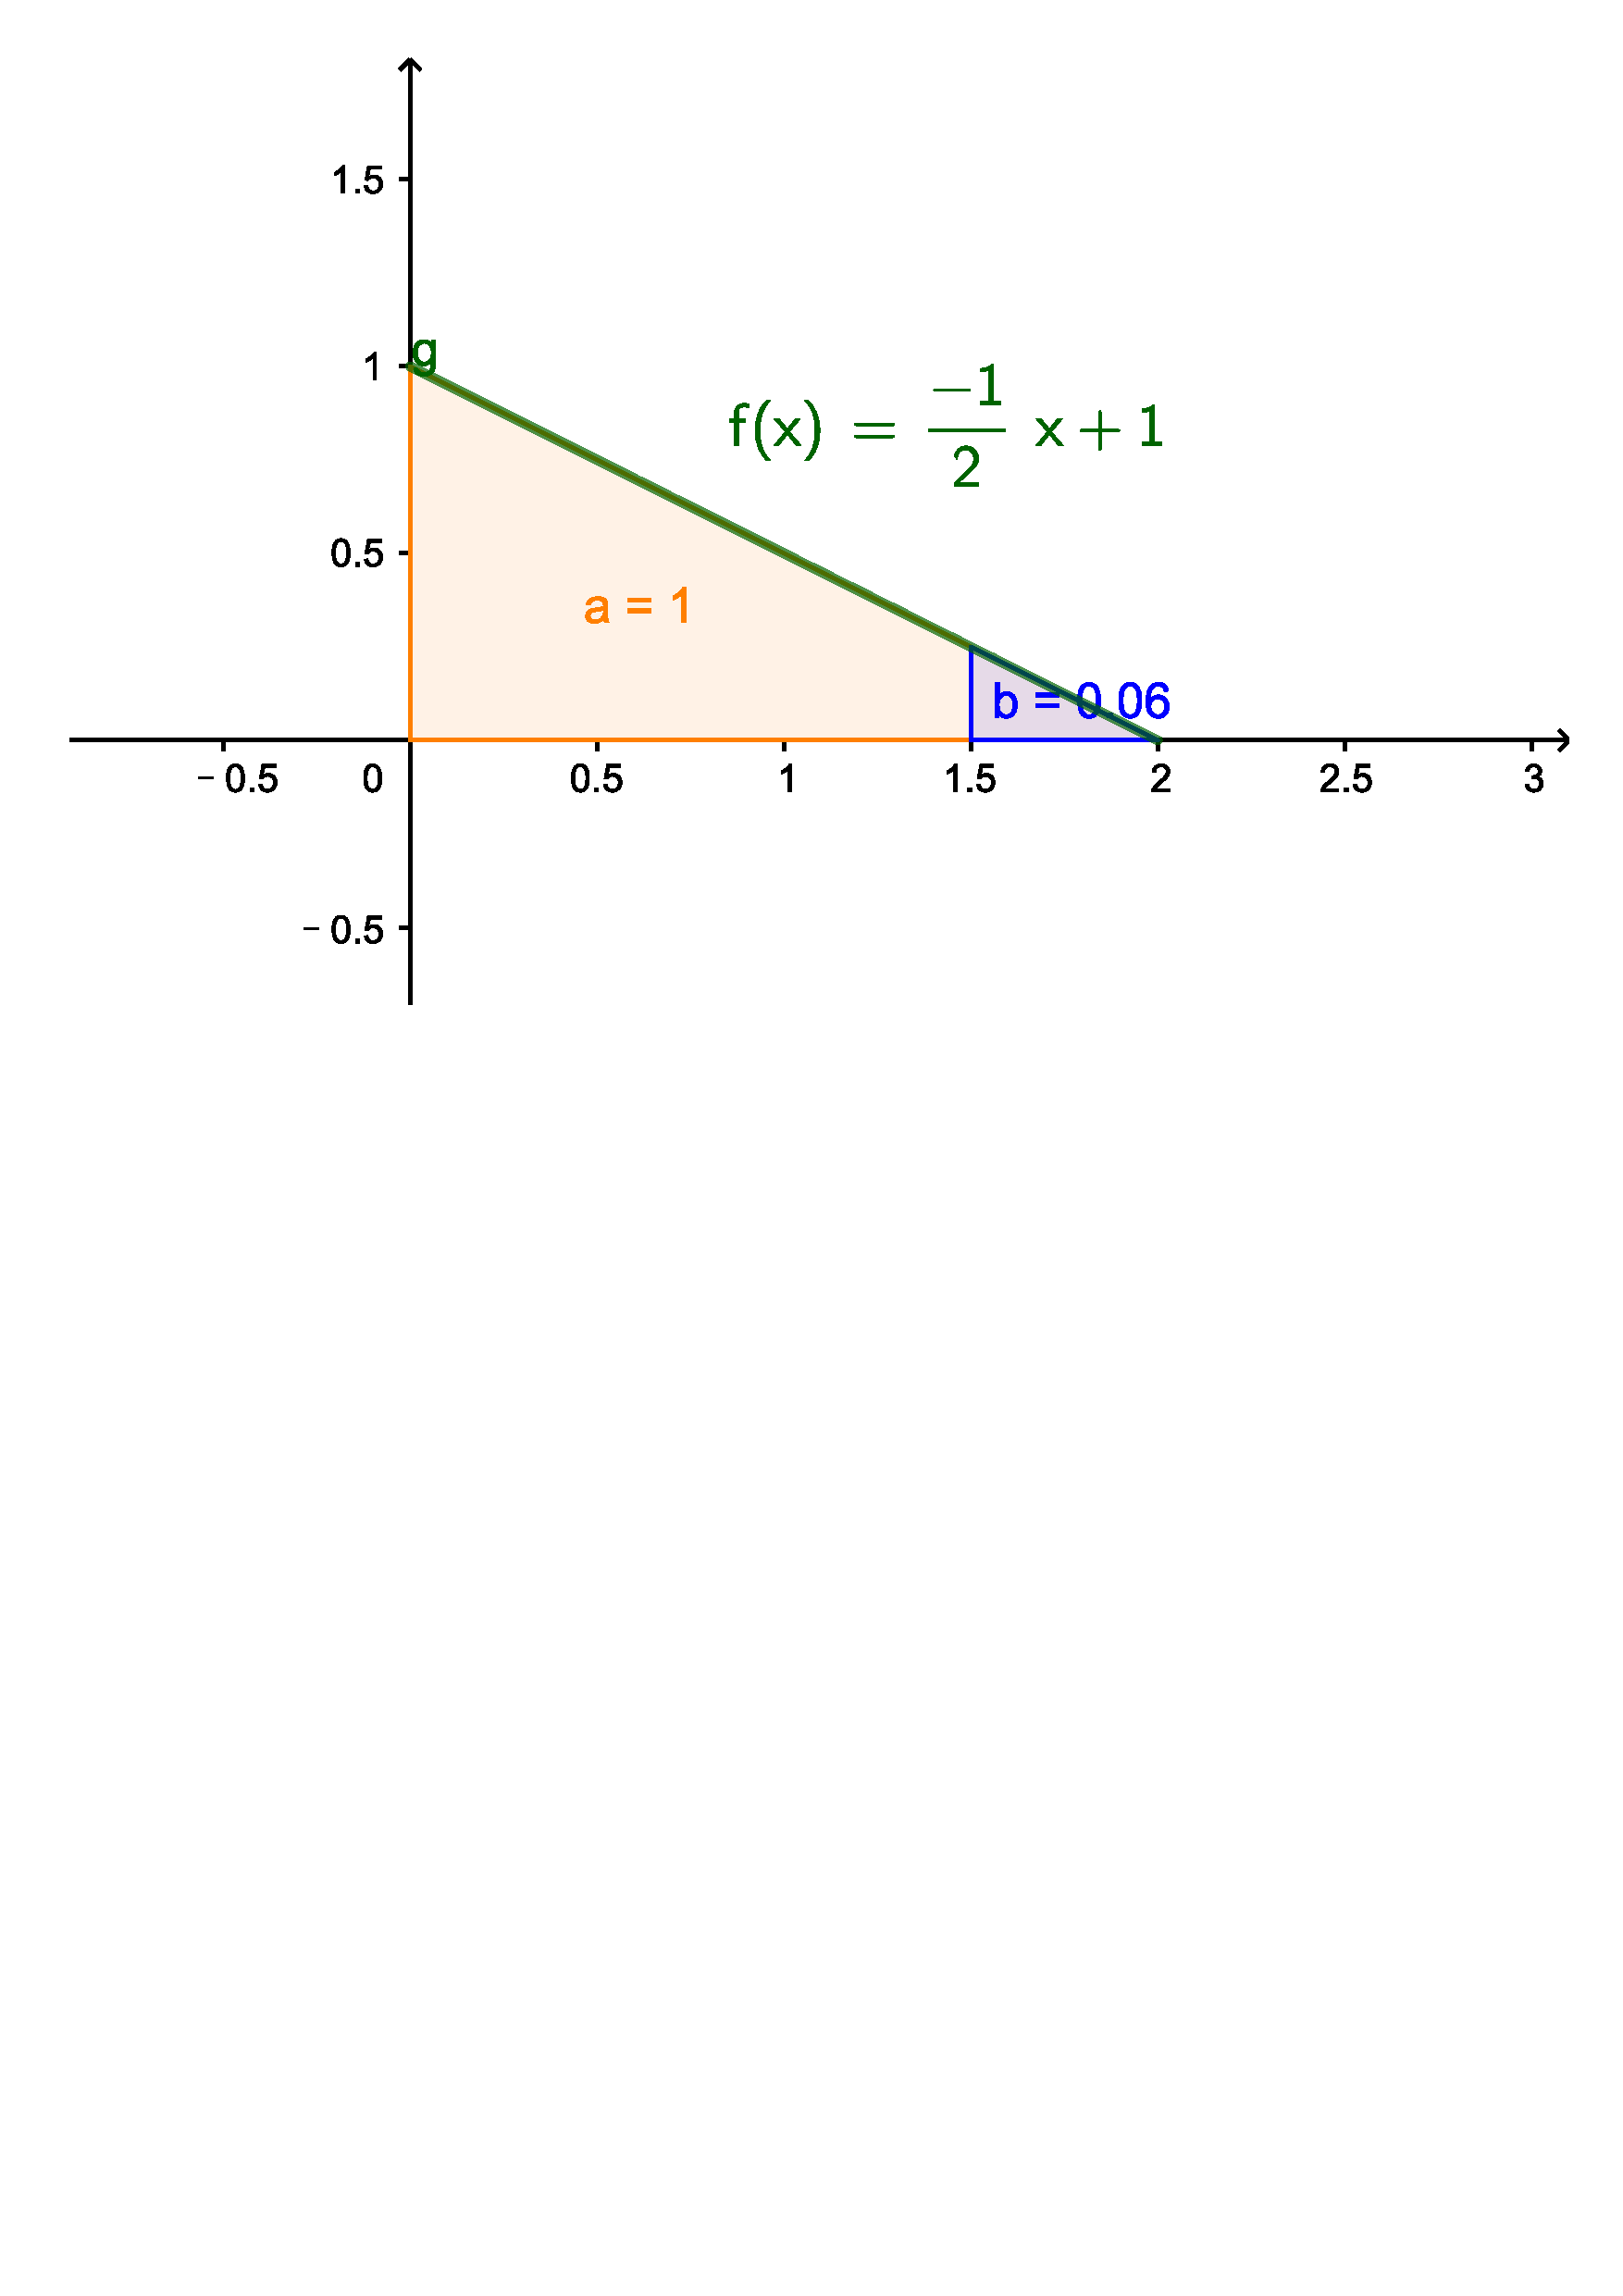
\includegraphics[width=0.6\textwidth]{/0127.pdf}
		
		
	\end{myEnvSample}
	
	
	
	
	\subsection{连续型随机变量, 取任一``个别值"的概率, 都为0.}
	
	比如, 在一段区间上, 投掷质点(无面积, 0维), 该质点砸中任何一个数值的概率, 就是为0. \\
	你可以倒过来想: 如果``该质点能砸中某个数值"的概率, 是可以给出的, 比如是 0.000001\%, 那``一段区间"上是有无穷多的点的, 0.000001\% 乘以无穷多, 一定是会超过 100\%的, 这就违反了概率不能超过1 的定义. 所以, ``质点投中任何位置处"的概率, 都无法给出, 是0. \\
	
	所以, 概率为0 的事件, 未必是``不可能事件". (如, 扔质子)  \\
	概率为1 的事件, 未必是``必然事件". 
	
	
	
	
	\subsection{如何求 PDF在某一x点处的y值(概率)?}
	
	
	\textbf{那么对于``连续性概率函数", 要求它在``x=某一点处"的概率, 该怎么求呢?  → 要用``极限"的概念来求.} \\
	
	即: 
	\begin{align*}  % 支持每行编号. 若不需要编号, 就用 align*环境
		&\lim_{\varDelta x\rightarrow 0}\frac{P\left\{ x<\text{随机变量}X<\left( x+\varDelta x \right) \right\}}{\varDelta x}\\
		&=\lim_{\varDelta x\rightarrow 0}\frac{\int_x^{x+\varDelta x}{f\left( x \right)}dx}{\varDelta x}\ \gets \text{分子分母是}\frac{0}{0}\text{型,用} \text{洛必达法则}”\text{来做}.\\
		&\text{即:}P\left\{ x<\text{随机变量}X<\left( x+\varDelta x \right) \right\} \approx \underset{y\text{高}}{\underbrace{f\left( x \right) }}\underset{x\text{宽}}{\underbrace{\varDelta x}}  
	\end{align*}
	
	所以, 千万不要误认为:``概率密度函数"在某一x点处的y值, 是该x点的概率. 事实上, \textbf{概率密度函数在某点的函数值, 是概率在该点的``变化率"(即斜率, 导数)!}  因为对于``连续性数据"来说, 任何一点的概率 都是0. 所以任何一点是不存在概率的! 我们只能得到"概率密度函数"在该x点处的斜率. 这个就类似于导数的概念. 导数代表着"该点处切线的斜率"! \\
	
	
	
	典型的``连续概率分布"包括: 正态分布, 指数分布等.
	
	
	
	
	
	
\end{document}